\section{Funcionamento do Oculus Rift}
O Oculus Rift é basicamente uma lente com uma tela de alta resolução juntamente com sensores e giroscópios trabalhando em conjunto. A sensação de imersão vem com a baixa taxa de resposta entre o movimento do usuário e a imagem gerada na tela, fazendo com que a experiência se torne algo prazeroso e confortável.

\subsection{Esquema de coordenadas}
Para manter a rastreabilidade dos movimentos da cabeça do usuário, o Oculus Rift trabalha com um sistema de coordenadas parecido com o da regra da mão direita. A figura abaixo ilustra como os eixos e sentidos são levados em consideração para o Rift.
\begin{itemize}
  \item Y é positivo para cima
  \item X é positivo para direita
  \item Z é positivo para traz
\end{itemize}
A rotação é mantida como uma unidade quaternária, mas também pode ser reportada na forma \textit{yaw-pitch-roll}. Os termos vêm do inglês e significam, respectivamente, giro, arremesso e rolo. Cada um dos eixos geram valores que significam as rotações (positivas ou negativas) de acordo com o movimento da cabeça do usuário:
\begin{itemize}
  \item \textit{Pitch} é a rotação entorno do eixo X, positivo quando arremessado para cima
  \item \textit{Yaw} é a rotação entorno do eixo Y , positivo quando virado para esquerda
  \item \textit{Roll} é a rotação entorno do eixo Z, positivo quando se encosta a cabeça no ombro esquerdo
\end{itemize}

\begin{figure}[h]
  \centering
  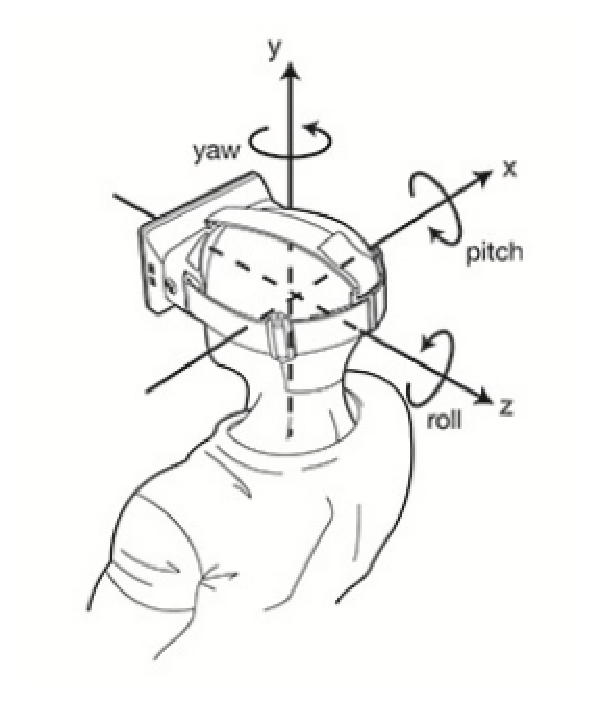
\includegraphics[width=0.5\textwidth]
      {figuras/esquema_coordenadas_rift.eps}
  \caption{Esquema de coordenadas do Oculus Rift}
  \label{coordenadas-rift}
\end{figure}

\subsection{Distorção}
O Oculus Rift requer que a cena seja renderizada em uma tela dividida com metade da tela usada para cada olho. Ao usar o aparelho, o olho esquerdo enxerga a metade esquerda da tela e o olho direito a metade direita. Por mais que varie de pessoa para pessoa, a distância das pupilas de um ser humano estão, aproximadamente, 65 mm longes uma da outra. Essa distância é conhecida como \textit{interpupillary distance}(IPD), ou distância interpupilar. Essa distância deve ser levada em consideração ao se escolher a distância entre as câmeras que captam as cenas na aplicação. Observe que o IPD se refere à translação da câmera, e não à rotação, e é essa translação que causa o efeito esteroscópico*. Isso significa que a sua aplicação precisará de renderizar a cena inteira duas vezes, uma para a metade esquerda e outra para a metade direita. 

As lentes do Oculus Rift ampliam a imagem para proporcionar grande \textit{field of view} (FOV), ou campo de visão, (quase total) que melhora muito a imersão virtual, basicamente não se vê outra coisa além do \"ambiente\" gerado pelas telas. Entretanto, as lentes distorcem a imagem final signicativamente até o ponto do usuário enxergar a distorção de almofada (distorcida \"para dentro\"). Para reverter a distorção da lente, deve haver a aplicação de um pós-processamento nas imagens renderizadas a fim de distorcê-las \"para fora\" (distorção de barril), figura abaixo. Sendo assim, os desenvolvedores implementaram uma API para aplicar distorção na imagem com o objetivo de ser cancelada pela lente do Rift. Finalmente, a API também trata o efeito chamado \"effeito arco-íris\" causado pelas bordas da lente. Mesmo que os parâmetros de distorção dependam das características da lente e da posição relativa dos olhos em relação a lente, a API cuida de todos os aspectos de geração da distorção, gerando uma imagem final no Oculus sem distorção alguma.

\begin{figure}[h]
  \centering
  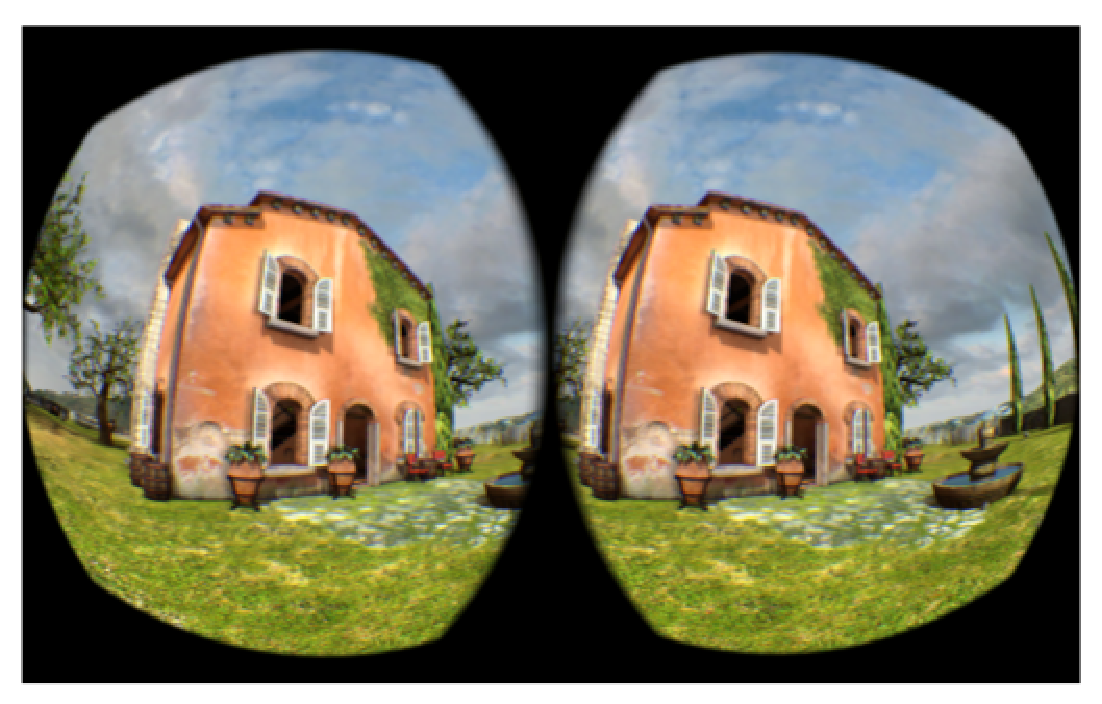
\includegraphics[width=0.7\textwidth]
      {figuras/distorcao_barril.eps}
  \caption{Imagem com distorção de barril}
  \label{coordenadas-rift}
\end{figure}

A projeção dos eixos das câmeras deve ser paralela uma com a outra como na figura abaixo. As vistas esquerda e direita são independentes uma da outra, isso significa que a configuração das câmeras da aplicação é basicamente a mesma ao se utilizar uma câmera única, a diferença é a distância entre os dois eixos ao se criar uma cena para o Rift.

\begin{figure}[h]
  \centering
  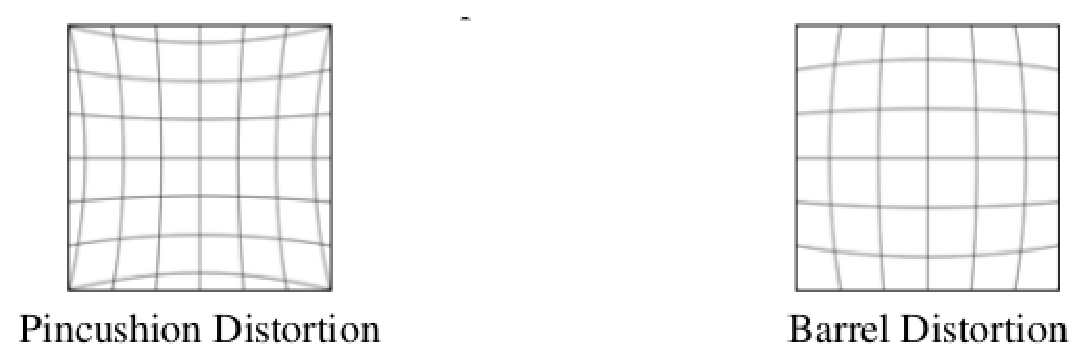
\includegraphics[width=0.7\textwidth]
      {figuras/distorcao_rift.eps}
  \caption{Distorção de lentes e imagens do Rift}
  \label{coordenadas-rift}
\end{figure}
